\documentclass[
	12pt,				% tamanho da fonte
	oneside,			% para impressão no anverso. Oposto a twoside
	a4paper,			% tamanho do papel. 
	chapter=TITLE,		% títulos de capítulos convertidos em letras maiúsculas
	section=TITLE,		% títulos de seções convertidos em letras maiúsculas
	english,			% idioma adicional para hifenização
	brazil  			% o último idioma é o principal do documento
	]{abntex2}

\usepackage{setup/ufscthesisA4-alf}
\usepackage{csquotes}
\usepackage[backend = biber, style = abnt]{biblatex}
\usepackage{graphicx}
\usepackage{color}
\usepackage{listings}
\usepackage{multirow}
\usepackage{tabularx}
\usepackage[table]{xcolor}
\usepackage{colortbl}
\usepackage{framed}
\usepackage{amssymb}
\usepackage{afterpage}
\usepackage{hhline}
\usepackage{enumitem}
\usepackage{latexsym}
\usepackage{lipsum}
\usepackage{setspace}
\usepackage{tabularray}

\definecolor{shadecolor}{rgb}{0.8,0.8,0.8}

\setlength\bibitemsep{\baselineskip}
\DeclareFieldFormat{url}{Disponível~em:\addspace\url{#1}}
\NewBibliographyString{sineloco}
\NewBibliographyString{sinenomine}
\DefineBibliographyStrings{brazil}{%
	sineloco     = {\mkbibemph{S\adddot l\adddot}},
	sinenomine   = {\mkbibemph{s\adddot n\adddot}},
	andothers    = {\mkbibemph{et\addabbrvspace al\adddot}},
	in			 = {\mkbibemph{In:}}
}

\addbibresource{aftertext/references.bib}

\DeclareSourcemap{
	\maps[datatype=bibtex]{
		\map{
			\step[fieldset=abstract, null]
			\step[fieldset=pagetotal, null]
		}
		\map{
			\pertype{inproceedings}
			\step[fieldset=venue, null]
			\step[fieldset=eventdate, null]
			\step[fieldset=eventtitle, null]
			\step[fieldset=isbn, null]
			\step[fieldset=volume, null]
		}
	}
}

% Definições gerais
\autor{Eric Fernandes Evaristo}
\titulo{Uso de uma MLLM para classificar lesões de pele}
\orientador[Orientador]{Aldo von Wangenheim, Prof. Dr. rer.nat.}  % TODO: Verificar os títulos
\ano{2024}
\local{Florianópolis}
\instituicaosigla{UFSC}
\instituicao{Universidade Federal de Santa Catarina}
\tipotrabalho{Proposta de Trabalho de Conclusão de Curso}
\formacao{Bacharel em Ciências da Computação}
\nivel{Bacharel}
\programa{Curso de Graduação em Ciências da Computação}
\centro{Centro Tecnológico}

\preambulo
{
\imprimirtipotrabalho~do~\imprimirprograma~do~\imprimircentro~da~\imprimirinstituicao~para~a~obtenção~do~título~de~\imprimirformacao.
}

% Configurações de aparência do PDF final
\definecolor{blue}{RGB}{41,5,195}
\makeatletter
\hypersetup{
		pdftitle={\@title},
		pdfauthor={\@author},
    	pdfsubject={\imprimirpreambulo},
	    pdfcreator={LaTeX with abnTeX2},
		pdfkeywords={ufsc, latex, abntex2},
		colorlinks=true,
    	linkcolor=black,
    	citecolor=black,
    	filecolor=black,
		urlcolor=black,
		bookmarksdepth=4
}
\makeatother

% Declaração das siglas
\siglalista{MLLMs}{\textit{Multimodal Large Language Models}}
\siglalista{LLM}{\textit{Large Language Model}}
\siglalista{LLaVa}{\textit{Large Language and Vision Assistant}}
\siglalista{CLIP ViT-L/14}{\textit{Contrastive Language-Image Pre-training ViT-L/14}}
\siglalista{PEFT}{\textit{Parameter-Efficient Fine-Tuning}}
\siglalista{LoRa}{\textit{Low-Rank Adaptation}}
\siglalista{TCC}{\textit{Trabalho de Conclusão de Curso}}

% Compila a lista de abreviaturas e siglas e a lista de símbolos
\makenoidxglossaries

% Compila o indice
\makeindex

% Início do documento
\begin{document}

% Seleciona o idioma do documento (conforme pacotes do babel)
%\selectlanguage{english}
\selectlanguage{brazil}

% Retira espaço extra obsoleto entre as frases.
\frenchspacing

% Espaçamento 1.5 entre linhas
\OnehalfSpacing

% Corrige justificação

% Elementos pré-textuais
% Capa
\imprimircapa

% Folha de rosto
% (o * indica que haverá a ficha bibliográfica)
\imprimirfolhaderosto

% Folha de aprovação
\begin{folhadeaprovacao}
	\small
	\begin{snugshade}
		\begin{center}
			{\textbf{FOLHA DE APROVAÇÃO DE PROPOSTA DE TCC}}
		\end{center}
	\end{snugshade}
	\vspace{-18pt}

	\footnotesize
	\begin{quadro}[htb]
		\centering
		\label{qua:folha_aprov}
		\begin{tabular}{|l|p{10.5cm}|}
			\hline
			\textbf{Acadêmico}            & \imprimirautor      \\ \hline
			\textbf{Título do trabalho}   & \imprimirtitulo     \\ \hline
			\textbf{Curso}                & \imprimirprograma   \\ \hline
			\textbf{Área de Concentração} & Visão computacional \\ \hline
		\end{tabular}
	\end{quadro}

	\vspace{-14pt}

	\noindent \textbf{Instruções para preenchimento pelo ORIENTADOR DO TRABALHO}:
	\begin{itemize}[leftmargin=*,noitemsep,topsep=0pt]
		\item[-] Para cada critério avaliado, assinale um X na coluna SIM apenas se considerado aprovado. Caso contrário, indique as alterações necessárias na coluna Observação.
	\end{itemize}

	\vspace{-4pt}

	\definecolor{Silver}{rgb}{0.752,0.752,0.752}
	\begin{table}[htb]
		\footnotesize
		\centering
		\begin{tblr}{
			width = \linewidth,
			colspec = {Q[452]Q[56]Q[85]Q[56]Q[150]Q[137]},
			row{1} = {Silver,c},
			row{2} = {Silver,c},
			cell{1}{1} = {r=2}{},
			cell{1}{2} = {c=4}{0.347\linewidth},
			cell{1}{6} = {r=2}{},
			cell{3}{2} = {Silver},
			cell{3}{3} = {Silver},
			cell{3}{4} = {Silver},
			cell{3}{5} = {Silver},
			cell{4}{2} = {Silver},
			cell{4}{3} = {Silver},
			cell{4}{4} = {Silver},
			cell{4}{5} = {Silver},
			cell{5}{2} = {Silver},
			cell{5}{3} = {Silver},
			cell{5}{4} = {Silver},
			cell{5}{5} = {Silver},
			cell{6}{2} = {Silver},
			cell{6}{3} = {Silver},
			cell{6}{4} = {Silver},
			cell{6}{5} = {Silver},
			cell{7}{2} = {Silver},
			cell{7}{3} = {Silver},
			cell{7}{4} = {Silver},
			cell{7}{5} = {Silver},
			cell{8}{2} = {Silver},
			cell{8}{3} = {Silver},
			cell{8}{4} = {Silver},
			cell{8}{5} = {Silver},
			cell{9}{2} = {Silver},
			cell{9}{3} = {Silver},
			cell{9}{4} = {Silver},
			cell{9}{5} = {Silver},
			cell{10}{2} = {Silver},
			cell{10}{3} = {Silver},
			cell{10}{4} = {Silver},
			cell{10}{5} = {Silver},
			cell{11}{2} = {Silver},
			cell{11}{3} = {Silver},
			cell{11}{4} = {Silver},
			cell{11}{5} = {Silver},
			cell{12}{2} = {Silver},
			cell{12}{3} = {Silver},
			cell{12}{4} = {Silver},
			cell{12}{5} = {Silver},
			cell{13}{2} = {Silver},
			cell{13}{3} = {Silver},
			cell{13}{4} = {Silver},
			cell{13}{5} = {Silver},
			cell{14}{2} = {Silver},
			cell{14}{3} = {Silver},
			cell{14}{4} = {Silver},
			cell{14}{5} = {Silver},
			cell{15}{2} = {Silver},
			cell{15}{3} = {Silver},
			cell{15}{4} = {Silver},
			cell{15}{5} = {Silver},
			vlines,
			hline{1,3-16} = {-}{},
					hline{2} = {2-5}{},
				}
			\textbf{Critérios }                                                                                                                                                                                                                                                                                & \textbf{Aprovado } &                  &              &                        & \textbf{Observação } \\
			                                                                                                                                                                                                                                                                                                   & \textbf{Sim}       & \textbf{Parcial} & \textbf{Não} & \textbf{Não se aplica} &                      \\
			{1. O trabalho é adequado para um TCC no CCO/SIN (relevância / abrangência)?}                                                                                                                                                                                                                      &                    &                  &              &                        &                      \\
			2. O titulo do trabalho é adequado?                                                                                                                                                                                                                                                                &                    &                  &              &                        &                      \\
			{3. O tema de pesquisa está claramente descrito?}                                                                                                                                                                                                                                                  &                    &                  &              &                        &                      \\
			{4. O problema/hipóteses de pesquisa do trabalho está claramente identificado?}                                                                                                                                                                                                                    &                    &                  &              &                        &                      \\
			5. A relevância da pesquisa é justificada?                                                                                                                                                                                                                                                         &                    &                  &              &                        &                      \\
			{6. Os objetivos descrevem completa e claramente o que se pretende alcançar neste trabalho?}                                                                                                                                                                                                       &                    &                  &              &                        &                      \\
			{7. É definido o método a ser adotado no trabalho? O método condiz com os objetivos e é adequado para um TCC?}                                                                                                                                                                                     &                    &                  &              &                        &                      \\
			{8. Foi definido um cronograma coerente com o método definido (indicando todas as atividades) e com as datas das entregas (p.ex. Projeto I, II, Defesa)?}                                                                                                                                          &                    &                  &              &                        &                      \\
			{9. Foram identificados custos relativos à execução deste trabalho (se houver)? Haverá financiamento para estes custos?}                                                                                                                                                                           &                    &                  &              &                        &                      \\
			{10. Foram identificados todos os envolvidos neste trabalho?}                                                                                                                                                                                                                                      &                    &                  &              &                        &                      \\
			{11. As formas de comunicação foram definidas (ex: horários para orientação)?}                                                                                                                                                                                                                     &                    &                  &              &                        &                      \\
			{12. Riscos potenciais que podem causar desvios do plano foram identificados?}                                                                                                                                                                                                                     &                    &                  &              &                        &                      \\
			{13. Caso o TCC envolva a produção de um software ou outro tipo de produto e seja desenvolvido também como uma atividade realizada numa empresa ou laboratório, consta da proposta uma declaração (Anexo 3) de ciência e concordância com a entrega do código fonte e/ou documentação produzidos?} &                    &                  &              &                        &
		\end{tblr}
	\end{table}

	\vspace{-4pt}

	\tiny
	\noindent \begin{tabularx}{\textwidth}{| l | X | l | l |}
		\hline
		{\textbf{Avaliação}}     & \multicolumn{1}{l}{\textbf{$\Box$ Aprovado}} & \multicolumn{2}{c|}{\textbf{$\Box$ Não Aprovado}}   \\ \hline
		{\textbf{Orientador}}    & {Prof. Dr. rer.nat. Aldo von Wangenheim}     & {00/00/2024}                                      & \\ \hline
		{\textbf{Co-orientador}} & {-}                                          & {00/00/2024}                                      & \\ \hline
	\end{tabularx}
\end{folhadeaprovacao}

% Resumo em português
\setlength{\absparsep}{18pt}
\begin{resumo}
	\SingleSpacing

	Lesões de pele podem ser um indicativo de diversas doenças, incluindo doenças graves como o câncer de pele. A detecção precoce dessas lesões é fundamental para o
	tratamento e cura da doença. Porém, o diagnóstico e classificação de uma lesão de pele é normalmente feita por profissionais especializados em hospitais ou clínicas.
	Isto pode levar a um atraso no diagnóstico pela falta de acesso ou procura pelo atendimento médico.

	Considerando este cenário, tecnologias como \ac{MLLMs} podem ser úteis. Estes modelos podem identificar lesões de pele com base em imagens e prover um pré-diagnóstico
	que pode alertar o portador da lesão sobre a necessidade de procurar atendimento médico. O modelo \ac{LLaVa} é um bom candidato para esta aplicação, pois consegue
	descrever imagens e pode ser adaptado para propósitos específicos.

	Neste trabalho, propõe-se a adaptação do \ac{LLaVa} com técnicas de \textit{fine tuning} para classificar lesões de pele com uma precisão aceitável.

	\textbf{Palavras-chave:} Lesões de pele. MLLM. LLaVa. Fine tuning. PEFT.
\end{resumo}

% Resumo em inglês (TODO)
%\begin{resumo}[Abstract]
%	\SingleSpacing
%	\begin{otherlanguage*}{english}
%		Resumo traduzido para outros idiomas, neste caso, inglês. Segue o formato do resumo feito na língua vernácula. As palavras-chave traduzidas, versão em língua estrangeira, são colocadas abaixo do texto precedidas pela expressão “Keywords”, separadas por ponto.

%		\textbf{Keywords}: Keyword 1. Keyword 2. Keyword 3.
%	\end{otherlanguage*}
%\end{resumo}

{
\hypersetup{hidelinks}

% Lista de siglas
\imprimirlistadesiglas

% Sumário
\pdfbookmark[0]{\contentsname}{toc}
\tableofcontents*
\cleardoublepage
}


% Elementos textuais
\textual

% 1 - Introdução
% ----------------------------------------------------------
\chapter{Introdução}
% ----------------------------------------------------------

%As orientações aqui apresentadas são baseadas em um conjunto de normas elaboradas pela \gls{ABNT}. Além das normas técnicas, a Biblioteca também elaborou uma série de tutoriais, guias, \textit{templates} os quais estão disponíveis em seu site, no endereço \url{http://portal.bu.ufsc.br/normalizacao/}.

%Paralelamente ao uso deste \textit{template} recomenda-se que seja utilizado o \textbf{Tutorial de Trabalhos Acadêmicos} (disponível neste link \url{https://repositorio.ufsc.br/handle/123456789/180829}) e/ou que o discente \textbf{participe das capacitações oferecidas da Biblioteca Universitária da UFSC}.

%Este \textit{template} está configurado apenas para a impressão utilizando o anverso das folhas, caso você queira imprimir usando a frente e o verso, acrescente a opção \textit{openright} e mude de \textit{oneside} para \textit{twoside} nas configurações da classe \textit{abntex2} no início do arquivo principal \textit{main.tex} \cite{abntex2classe}.

%Os trabalhos de conclusão de curso (TCC) de graduação e de especialização não são entregues em formato impresso na Biblioteca Universitária. Porém, sua versão PDF pode ser disponibilizada no Repositório Institucional, consulte seu curso sobre os procedimentos adotados para a entrega. 

%\nocite{NBR6023:2002}
%\nocite{NBR6027:2012}
%\nocite{NBR6028:2003}
%\nocite{NBR10520:2002}

% ----------------------------------------------------------
%\section{Recomendações de uso}
% ----------------------------------------------------------

%Este \emph{template} foi elaborado para se compilado em \LaTeX utilizando \abnTeX.  Todas as configurações de diferenciação gráfica nas divisões de seção e subseção seguem a  norma NBR 6027/2012 automaticamente. 

%Uma nota de rodapé, já tem seu estilo automático com o comando \texttt{$\backslash$footnote}\footnote{As notas de rodapé possuem fonte tamanho 10. O alinhamento das linhas da nota de rodapé deve ser abaixo da primeira letra da primeira palavra da nota de modo dar destaque ao expoente.}.

O consumo e compartilhamento de conteúdos em vídeo vem aumentando consideravelmente nos últimos anos.
Atualmente se estima que vídeos sejam responsáveis por 71\% de todo o tráfego de dados móveis, e a previsão é que esse valor aumente para 80\% até 2028 \cite{mobile}.
Ao se considerar um panorama mais amplo, há dados apontando que conteúdo em vídeo representou quase 66\% do volume total de tráfego na Internet no primeiro semestre de 2022 \cite{traffic}, havendo aumento de 24\% em relação ao mesmo período de 2021.

Tendo em vista esse cenário, fica evidente a importância da codificação de vídeos, a qual busca formas de armazenar, transmitir e reproduzir esse tipo de dado de forma otimizada.
Nesse contexto, a abordagem mais consolidada é a codificação híbrida, a qual vem sendo parte essencial do estado da arte da área nas últimas décadas.
Os padrões de codificação híbridos valem-se de diferentes técnicas para examinar quadros e regiões dentro dos quadros a procura de informações redundantes para o sistema visual humano. Com isso, eles exploram a taxa de compressão atingida para minimizar tanto quanto possível o armazenamento, mantendo ao máximo a qualidade.
Contudo, o aumento da demanda e da concorrência observado recentemente tem levado ao desenvolvimento de algoritmos cada vez mais complexos, impactando no custo computacional e no tempo de execução.
Dessa maneira, a cada geração, a eficiência de codificação vem duplicando, ao custo de um aumento na complexidade de cerca de 10X.
Por consequência, técnicas alternativas têm sido propostas para tentar melhorar a eficiência de codificação, e uma delas é o \ac{DIVC} \cite{ours}.
Esse modelo de codificação consiste em combinar o uso de um dos padrões híbridos com a realização de \ac{VFI}.

\ac{VFI} é uma técnica para gerar ao menos um quadro intermediário ($Q_t$), tomando como referência pelo menos um quadro anterior ($Q_0$) e um posterior ($Q_1$), como mostra a Figura \ref{fig:vfi}.
Nesse caso, \textit{t} representa a posição temporal do quadro interpolado em relação aos quadros de referência, com $0<t<1$.
Os quadros podem ser produzidos com diferentes propósitos, e as implementações mais recentes são baseadas na utilização de \acp{NN}.
Uma das abordagens mais empregadas pode ser classificada como \textit{flow-based}, e consiste em computar o \textit{optical flow}, o qual é usado para relizar \textit{warping} sobre os quadros de referência.
Um exemplo desse tipo de arquitetura foi proposto por \textcite{niklaus2020softmax}.

\begin{figure}[htb]
    \centering
    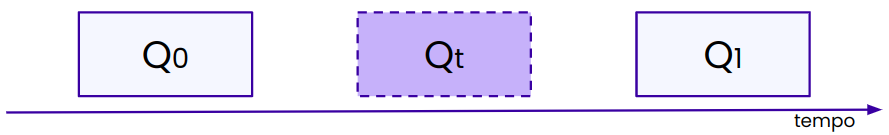
\includegraphics[width=0.8\columnwidth,keepaspectratio]{images/vfi1.png}
    \caption{Interpolação de Quadros de Vídeo - \textit{Video Frame Interpolation} (VFI). Fonte: Elaborado pela autora.}
    \label{fig:vfi}
\end{figure}

Dessa forma, a abordagem \ac{DIVC} propõe retirar os quadros de índice par do vídeo (riscados em vermelho na Figura \ref{fig:divc}) e codificar os quadros de índice ímpar com o método tradicional. Após a etapa de decodificação, \ac{VFI} é usado para regerar os quadros pares a partir dos quadros ímpares reconstruídos. Entretanto, um problema relacionado à aplicação dessa técnica que se observa a partir dos testes realizados é que os resultados variam muito em função do conteúdo do vídeo \cite{ours}.

\begin{figure}[htb]
    \centering
    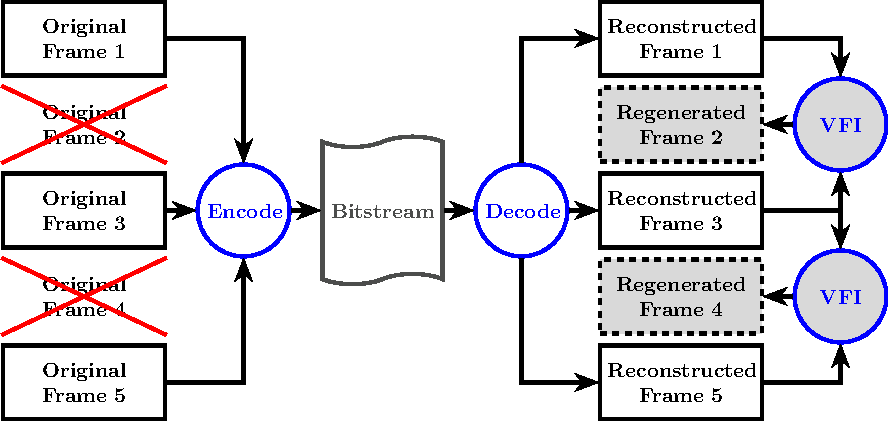
\includegraphics[width=0.8\columnwidth,keepaspectratio]{images/hybrid_vfi.pdf}
    \caption{\textit{Decoupled Interpolated Video Coding} (DIVC). Fonte: \textcite{ours}.}
    \label{fig:divc}
\end{figure}

Um tipo de ferramenta que pode ser útil para identificar características e conteúdos presentes em imagens e vídeos são os descritores \cite{Kumar2014ASO}. Eles podem ser utilizados para inúmeras aplicações, como reconhecimento de padrões, rastreamento e identificação de objetos. Um exemplo de descritor conhecido na literatura é o \ac{ORB} \cite{orb}, que foi desenvolvido tendo como foco diversas aplicações, como detecção de objetos e \textit{patch-tracking}. Outro exemplo é o \ac{FREAK} \cite{freak}, o qual foi projetado tendo inspiração no \ac{SVH}.

Assim, especula-se que seja possível melhorar a eficiência de codificação do \ac{DIVC} a partir da remoção de quadros de maneira adaptativa. Essa remoção poderia ser feita considerando características do conteúdo, as quais seriam obtidas com o auxílio de descritores de imagem e/ou vídeo.

%Inicialmente nesse relatório discute-se sobre o referencial teórico básico dos algoritmos de aprendizado de máquina que foram utilizados, juntamente com a explicação dos cálculos matemáticos que são feitos nas predições dos modelos. Depois, explicam-se os métodos utilizados para se extrair os dados que treinaram os algoritmos, assim como as técnicas aplicadas em suas modelagens para evitar problemas de \textit{overfit} e melhorar a performance dos modelos tomando como base a função de custo escolhida. Logo em seguida os resultados dos treinamentos são discutidos por meio tanto da análise dos erros da predições quanto pela representação gráfica mais intuitiva desses erros. Por fim, sintetiza-se todo o processo realizado e os resultados obtidos em uma conclusão que indica qual foi o melhor algoritmo e o pior algoritmo para o objetivo posto nesse trabalho. 


% ----------------------------------------------------------
\section{Objetivos}
% ----------------------------------------------------------

%Nas seções abaixo estão descritos o objetivo geral e os objetivos específicos deste TCC.

% ----------------------------------------------------------
% São objetivos gerais e especificos deste trabalho: 


% \subsection*{Objetivo Geral}
% % ----------------------------------------------------------

%Neste panorama, este trabalho de conclusão de curso tem dois objetivos principais. Em primeiro momento, propõe-se a utilizar técnicas de \gls{AxC} para desenvolver e avaliar um conjunto de comparadores aproximados seguindo figuras de mérito estabelecidos na literatura. Posteriormente, busca fornecer um fluxo de projeto para determinação das técnicas de aproximação mais apropriadas para comparadores no contexto de aplicações de classificação com \gls{DT}s, de modo a otimizar a relação entre dissipação de potência e acurácia.

O objetivo geral deste trabalho é melhorar a eficiência de codificação do modelo \ac{DIVC} através da remoção de quadros de vídeos de forma adaptativa.
Para essa finalidade, pretende-se utilizar diferentes descritores de imagem e/ou vídeo para extrair características das sequências as quais tenham potencial influência na qualidade dos resultados obtidos com a aplicação do \ac{DIVC}.


% ----------------------------------------------------------
\subsection*{Objetivos Específicos}
% ----------------------------------------------------------

\begin{itemize}
    \item Determinar quais descritores de imagem/vídeo apresentam melhor correlação com a eficiência de codificação na utilização do método \ac{DIVC};
    \item Melhorar a eficiência de codificação do modelo \ac{DIVC} através da remoção adaptativa de quadros, a partir da avaliação dos mesmos por meio dos descritores escolhidos.
\end{itemize}
% ----------------------------------------------------------	


% 2 - Capítulo 2
\chapter{Planejamento}

Este capítulo trata do método de pesquisa e desenvolvimento do projeto, incluindo o cronograma, orçamento, recursos humanos necessários, definições sobre comunicação e
riscos associados.

\section{Método de Pesquisa}

A execução do projeto será caracterizada por uma parte teórica de pesquisa do estado da arte e de tecnologias utilizáveis e por uma parte prática em que o modelo será
desenvolvido e testado. Além disso, o trabalho será feito com o auxílio de um grupo de pesquisa de \ac{MLLMs}.

A primeira etapa do projeto se consistirá no estudo do estado da arte de \ac{MLLMs} e do processo de treinamento destes modelos. Além disso, serão estudadas as técnicas
de \textit{fine tuning} com um foco em \ac{PEFT} e suas aplicações no \ac{LLaVa}.

A próxima etapa se consiste em uma análise do conjunto de dados a ser utilizado, de modo a tratá-lo para a sua utilização no desenvolvimento.

Posteriormente será feito o \textit{fine tuning} do modelo \ac{LLaVa} com diferentes métodos, visando a eficiência do processo. Nesta etapa também serão feitos testes
para avaliar a precisão do modelo resultante.

Por fim, será feita uma análise dos resultados com o propósito de determinar a viabilidade da utilização do modelo resultante para a classificação de lesões de pele.

\pagebreak

\section{Cronograma}

\vspace{-1cm}

\definecolor{Silver}{rgb}{0.752,0.752,0.752}
\noindent \begin{table}[htb]
	\centering
	\begin{tblr}{
		width = \linewidth,
		colspec = {Q[371]Q[37]Q[46]Q[38]Q[40]Q[44]Q[44]Q[44]Q[40]Q[46]Q[40]Q[46]Q[44]Q[37]},
		row{1} = {Silver,c},
		row{2} = {Silver},
		cell{1}{1} = {r=2}{},
		cell{1}{2} = {c=13}{0.545\linewidth},
		cell{2}{2} = {c},
		cell{2}{3} = {c},
		cell{2}{4} = {c},
		cell{2}{5} = {c},
		cell{3}{2} = {Silver},
		cell{3}{3} = {Silver},
		cell{4}{3} = {Silver},
		cell{4}{4} = {Silver},
		cell{5}{4} = {Silver},
		cell{5}{5} = {Silver},
		cell{6}{6} = {Silver},
		cell{6}{7} = {Silver},
		cell{6}{8} = {Silver},
		cell{6}{9} = {Silver},
		cell{7}{6} = {Silver},
		cell{7}{7} = {Silver},
		cell{8}{9} = {Silver},
		cell{8}{10} = {Silver},
		cell{8}{11} = {Silver},
		cell{8}{12} = {Silver},
		cell{9}{12} = {Silver},
		cell{9}{13} = {Silver},
		cell{10}{13} = {Silver},
		cell{11}{14} = {Silver},
		vlines,
		hline{1,3-12} = {-}{},
				hline{2} = {2-14}{},
			}
		\textbf{Etapas}                                                                             & \textbf{Meses} &             &             &             &             &             &             &             &             &             &             &             &             \\
		                                                                                            & \textbf{07}    & \textbf{08} & \textbf{09} & \textbf{10} & \textbf{11} & \textbf{12} & \textbf{01} & \textbf{02} & \textbf{03} & \textbf{04} & \textbf{05} & \textbf{06} & \textbf{07} \\
		Estudo da fundamentação teórica dos \ac{MLLMs} e dos métodos de treinamento                 &                &             &             &             &             &             &             &             &             &             &             &             &             \\
		Estudo da utilização de métodos de \textit{fine tuning} baseados em \ac{PEFT} no \ac{LLaVa} &                &             &             &             &             &             &             &             &             &             &             &             &             \\
		Análise e tratamento do conjunto de dados                                                   &                &             &             &             &             &             &             &             &             &             &             &             &             \\
		\textit{Fine tuning}~do \ac{LLaVa} com diferentes métodos                                   &                &             &             &             &             &             &             &             &             &             &             &             &             \\
		Entrega do relatório do \ac{TCC} I                                                          &                &             &             &             &             &             &             &             &             &             &             &             &             \\
		Testes e análise dos modelos resultantes                                                    &                &             &             &             &             &             &             &             &             &             &             &             &             \\
		Entrega do relatório do \ac{TCC} II                                                         &                &             &             &             &             &             &             &             &             &             &             &             &             \\
		Defesa pública                                                                              &                &             &             &             &             &             &             &             &             &             &             &             &             \\
		Ajustes finais no relatório do \ac{TCC}                                                     &                &             &             &             &             &             &             &             &             &             &             &             &
	\end{tblr}
\end{table}

\section{Custos}

\noindent \begin{tabular} {|X p{4cm}|c|c|c|}
	\hline
	{\cellcolor{shadecolor}} \textbf{Item}          & {\cellcolor{shadecolor}} \textbf{Quantidade} & {\cellcolor{shadecolor}} \textbf{Valor Unitário (R\$)} & {\cellcolor{shadecolor}} \textbf{Total (R\$)} \\ \hline
	\hline
	\multicolumn{4}{|c|}{Material de Consumo}                                                                                                                                                               \\ \hline
	Assinatura mensal de internet 350 Gb/s          & 12                                           & $100$                                                  & $1200,00$                                     \\ \hline
	Assinatura mensal do Google Colab Pro           & 12                                           & $58$                                                   & $696,00$                                      \\ \hline
	\hline
	\multicolumn{4}{|c|}{Outros recursos e serviços}                                                                                                                                                        \\ \hline
	\multicolumn{4}{|c|}{Reserva de Contingência}                                                                                                                                                           \\ \hline
	Mitigação da falha da placa de vídeo (RTX 3060) &                                              &                                                        & $2600,00$                                     \\ \hline
	\hline
	\multicolumn{4}{|c|}{Total}                                                                                                                                                                             \\ \hline
	                                                &                                              &                                                        & $4496,00$                                     \\ \hline
\end{tabular}

\section{Recursos Humanos}

\noindent \begin{tabular}{|c|c|}
	\arrayrulecolor{white}
	\hline
	\arrayrulecolor{black}
	\hline
	\rowcolor{shadecolor}
	\textbf{Nome}           & \textbf{Função}         \\ \hline
	Eric Fernandes Evaristo & Autor                   \\ \hline
	Aldo von Wangenheim     & Orientador              \\ \hline
	-                       & Co-orientador           \\ \hline
	-                       & Membro da Banca         \\ \hline
	Renato Cislaghi         & Coordenador de Projetos \\ \hline
\end{tabular}

\section{Comunicação}

\noindent \resizebox{ \textwidth}{!}{
	\begin{tabular}{|X p{3cm}|X p{3cm}|X p{3cm}|X p{3cm}|X p{3cm}|}
		\hhline{|*{5}{-|}}
		{\cellcolor{shadecolor}} \textbf{O que precisa ser comunicado} & {\cellcolor{shadecolor}} \textbf{Por quem} & {\cellcolor{shadecolor}} \textbf{Para quem} & {\cellcolor{shadecolor}} \textbf{Melhor forma de Comunicação} & {\cellcolor{shadecolor}} \textbf{Quando e com que frequência} \\ \hhline{|*{5}{-|}}
		Ante-Projeto                                                   & Autor                                      & Coordenador de Projetos                     & Via site de projetos                                          & Ao fim de Cada Semestre                                       \\ \hhline{|*{5}{-|}}
		Orientação                                                     & Autor                                      & Orientador                                  & E-mail, Google Chat e videoconferência                        & Conforme for necessário                                       \\ \hhline{|*{5}{-|}}
		Acompanhamento do progresso do \ac{TCC}                        & Autor                                      & Orientador                                  & Videoconferência                                              & Bissemanalmente                                               \\ \hhline{|*{5}{-|}}
		Revisão do \ac{TCC}                                            & Autor                                      & Orientador                                  & Documento entregue por e-mail                                 & Próximo de cada entrega                                       \\ \hhline{|*{5}{-|}}
		Apresentação do \ac{TCC}                                       & Autor                                      & Orientador, membros da banca                & Via site de projetos e videoconferência                       & Ao fim do projeto                                             \\ \hhline{|*{5}{-|}}
	\end{tabular}
}

\section{Riscos}

\noindent\resizebox{\textwidth}{!}{
	\begin{tabular}{|X p{2cm}|c|c|c|X p{3cm}|X p{3cm}|}
		\hhline{|*{6}{-|}}
		{\cellcolor{shadecolor}} \textbf{Risco} & {\cellcolor{shadecolor}} \textbf{Probabilidade} & {\cellcolor{shadecolor}} \textbf{Impacto} & {\cellcolor{shadecolor}} \textbf{Prioridade} & {\cellcolor{shadecolor}} \textbf{Estratégia de Resposta} & {\cellcolor{shadecolor}} \textbf{Ações Preventivas}     \\ \hhline{|*{6}{-|}}
		Alteração no Tema                       & baixa                                           & alto                                      & alta                                         & Modificar o escopo do projeto atual                      & Garantir a viabilidade do tema com o orientador         \\ \hhline{|*{6}{-|}}
		Atraso nas entregas                     & baixa                                           & alto                                      & alta                                         & Replanejar                                               & Manter o cronograma realista e tolerante á adversidades \\ \hhline{|*{6}{-|}}
		Falha na placa de vídeo                 & baixa                                           & alto                                      & alta                                         & Adquirir uma nova placa de vídeo                         & Evitar o mau uso da placa de vídeo                      \\ \hhline{|*{6}{-|}}
	\end{tabular}
}


% 3 - Capítulo 3
% % ----------------------------------------------------------
\chapter{Seção}
% ----------------------------------------------------------

Este \textit{template} contém algumas seções criadas na tentativa de facilitar seu uso. No entanto, não há um limite máximo ou mínimo de seção a ser utilizado no trabalho. Cabe a cada autor definir a quantidade que melhor atenda à sua 
necessidade.  

% 4 - Conclusão
%\phantompart
% % ----------------------------------------------------------
\chapter{Conclusão}
% ----------------------------------------------------------

As conclusões devem responder às questões da pesquisa, em relação aos objetivos e às hipóteses. Devem ser breves, podendo apresentar recomendações e sugestões para trabalhos futuros.

% Elementos pós-textuais
\postextual

% Referências bibliográficas
\begingroup
\printbibliography[title=REFERÊNCIAS]
\endgroup


% Apêndices
%\begin{apendicesenv}
%	\partapendices* 
%	% ----------------------------------------------------------
\chapter{Descrição}
% ----------------------------------------------------------

Textos elaborados pelo autor, a fim de completar a sua argumentação. Deve ser precedido da palavra APÊNDICE, identificada por letras maiúsculas consecutivas, travessão e pelo respectivo título. Utilizam-se letras maiúsculas dobradas quando esgotadas as letras do alfabeto.

\begin{quadro}[htb]
    \centering
    \caption{\label{qua:Quadro_2}Modelo A.}
    \begin{tabular}{|l|l|}
        \hline
        xxxx              & yyyyyyyyyyyyyyy    \\
        \hline
        xxxx              & yyyyyyyyyyyyyyy    \\
        \hline
        xxxx              & yyyyyyyyyyyyyyy    \\
        \hline
        xxxx              & yyyyyyyyyyyyyyy    \\
        \hline
        xxxx              & yyyyyyyyyyyyyyy    \\
        \hline
        xxxx              & yyyyyyyyyyyyyyy    \\
        \hline
        xxxx              & yyyyyyyyyyyyyyy    \\
        \hline
        rrrrrrrrrrrrrrrrr & eeeeeeeeeeeeeeeee  \\
        \hline
        xxxx              & yyyyyyyyyyyyyyy    \\
        \hline
        xxxx              & yyyyyyyyyyyyyyy    \\
        \hline
        rrrrrrrrrrrrrrrrr & eeeeeeeeeeeeeeeee  \\
        \hline
        xxxx              & yyyyyyyyyyyyyyy    \\
        \hline
                          & ttttttttttttttttt  \\
        \hline
        rrrrrrrrrrrrrrrrr & eeeeeeeeeeeeeeeee  \\
        \hline
        ttttttttttttt     &                    \\
        \hline
        rrrrrrrrrrrrrrrrr & eeeeeeeeeeeeeeeee  \\
        \hline
        rrrrrrrrrrrrrrrrr & eeeeeeeeeeeeeeeee  \\
        \hline
                          & gggggggggggggggggg \\
        \hline
        rrrrrrrrrrrrrrrrr & eeeeeeeeeeeeeeeee  \\
        \hline
        rrrrrrrrrrrrrrrrr & eeeeeeeeeeeeeeeee  \\
        \hline
        rrrrrrrrrrrrrrrrr & eeeeeeeeeeeeeeeee  \\
        \hline
        rrrrrrrrrrrrrrrrr & eeeeeeeeeeeeeeeee  \\
        \hline
    \end{tabular}
    \fonte{Elaborada pelo autor (2016).}
\end{quadro}
%\end{apendicesenv}

\end{document}
